\documentclass[a4paper,11pt]{article}
\usepackage{amsmath}
%\usepackage[utf8]{inputenc}
\usepackage[T1]{fontenc}
\usepackage{graphicx}
\usepackage{titling}
\usepackage{listings}
\usepackage{hyperref}
\usepackage{float}
\usepackage{amsmath}
\usepackage{emoji}
\usepackage{minted}
\usepackage{pdfpages}
\usepackage[title]{appendix}
\hypersetup{
    colorlinks=true,
    linkcolor=magenta,
    citecolor=cyan,      
    urlcolor=cyan,
}
\lstset{%
  basicstyle=\scriptsize\sffamily,%
  commentstyle=\footnotesize\ttfamily,%
  frameround=trBL,
  frame=single,
  breaklines=true,
  showstringspaces=false,
  numbers=left,
  numberstyle=\tiny,
  numbersep=10pt,
  keywordstyle=\bf
}
\newcommand{\subtitle}[1]{%
  \posttitle{%
    \par\end{center}
    \begin{center}\large#1\end{center}
    \vskip0.5em}%
}
%\title{\vspace{-3.0cm}Final Year Project – Interim Report}
%\subtitle{CSU44099}
%\author{Eoin Brereton Hurley}
%\date{20/01/2023}
%\pagenumbering{gobble}
\begin{document}

%\maketitle
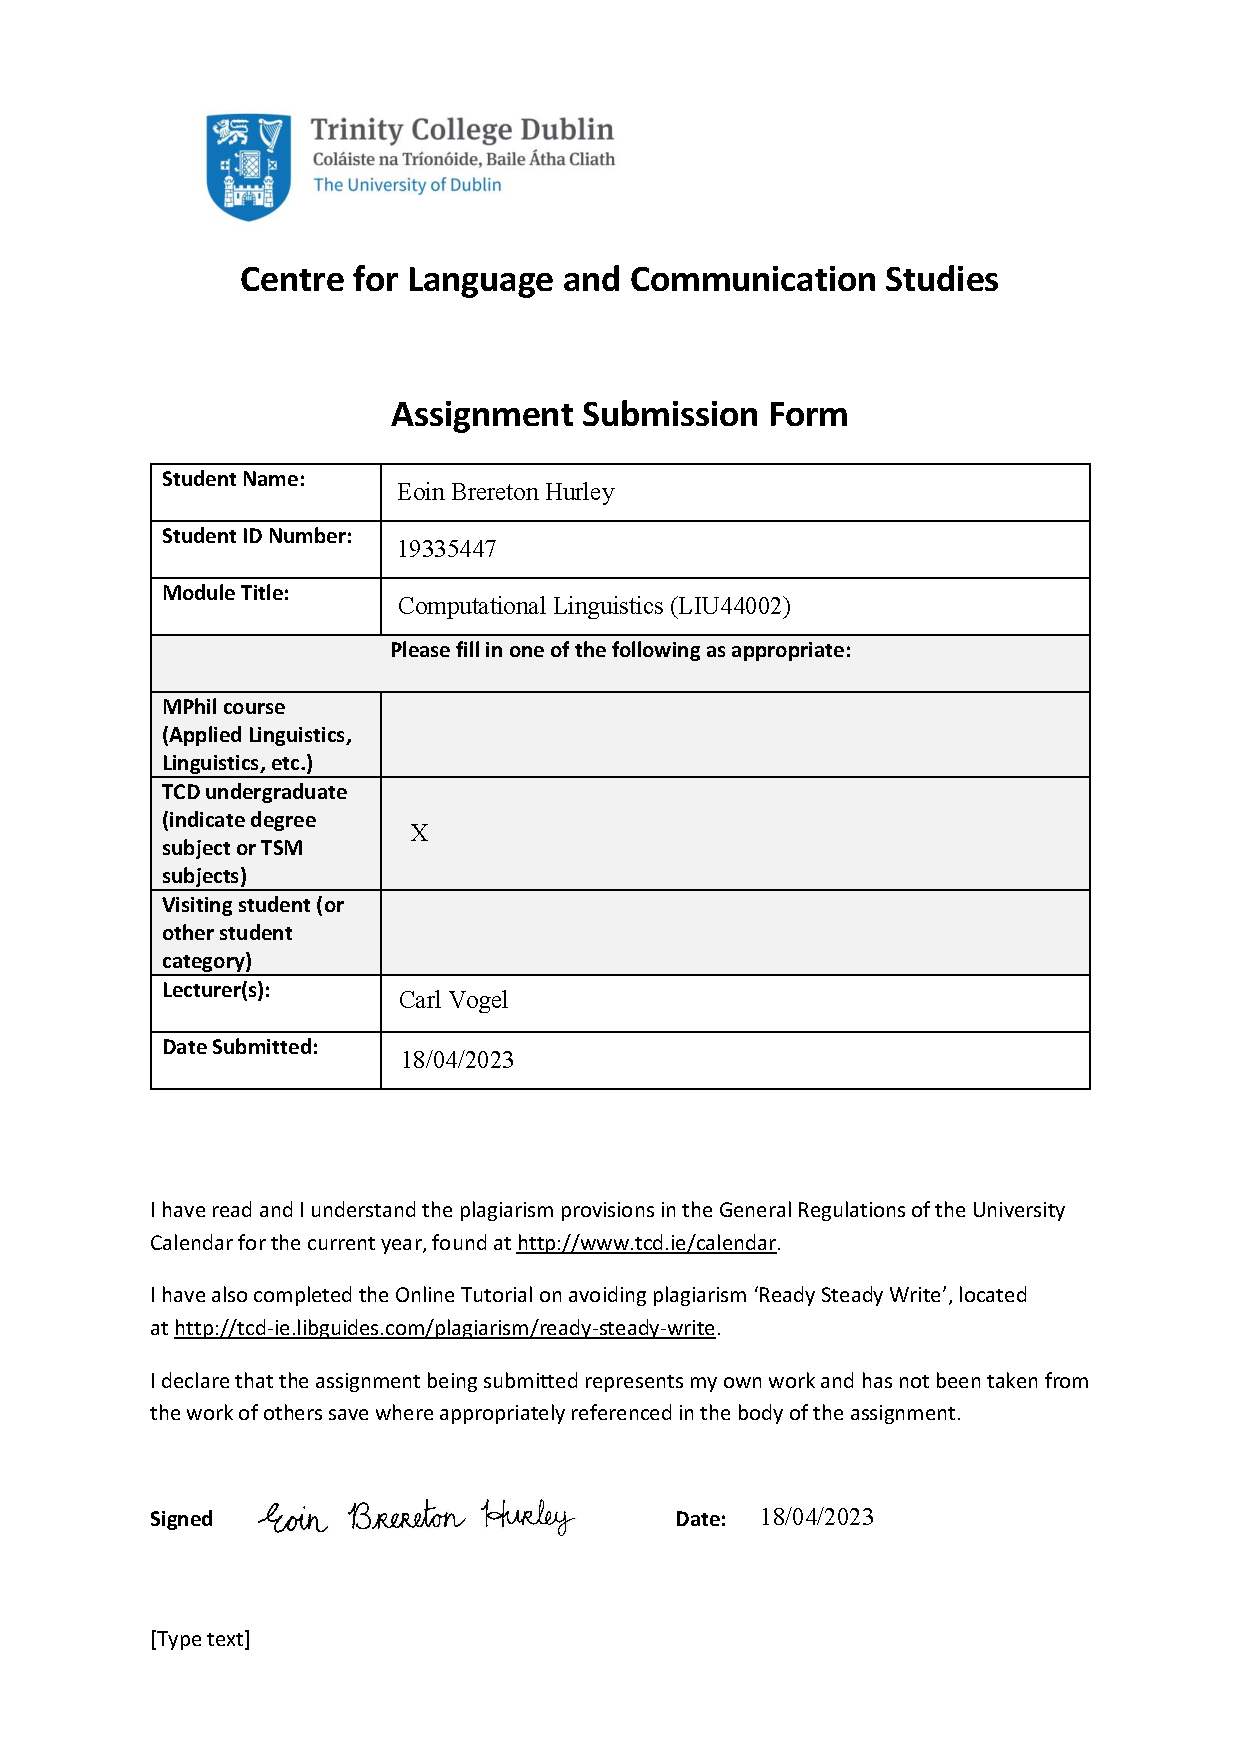
\includepdf[pages=-]{Declaration.pdf}
\begin{titlepage}
    \begin{center}
        \vspace*{1cm}
            
        \Huge
        \textbf{Exploring Linguistic Complexity of a TD (\textit{Teachta Dála})}
            
        \vspace{0.5cm}
        \LARGE
        LIU44002
        
        \vspace{0cm}
        
        \large
        Lecturer: Carl Vogel
        \vspace{1.5cm}
            
        \textbf{Eoin Brereton Hurley}

        \vspace{0.2cm}
        
        \large \today

        \vspace{0.2cm}
        
        \large 
            
        \vspace{2.0cm}
            
        
\includegraphics[width=1.0\textwidth]{tcd-logo.jpeg}

        \vfill
            
    \end{center}
\end{titlepage}
%\begin{abstract}
%Abstract
%\end{abstract}
\newcommand{\Tau}{\mathrm{T}}

\section{Introduction}
This essay concerns an investigation into the lexical and structural complexity of linguistic data produced by a TD (Teachta Dála) in the Irish government. The linguistic data in question comprises both social media posts and records of governmental proceedings obtained from \textit{Twitter} and \url{https://www.oireachtas.ie} respectively.

\subsection{Teachta Dála (TD) of Focus}
\subsubsection{Minister details:}
\paragraph{}
The selected TD of focus is Catherine Martin (born 30 September 1972): the Minister for Tourism, Culture, Arts, Gaeltacht, Sport and Media. As a member of the Green Party, this Minister operates out of the Dublin Rathdown consituency, which is located in the South Dublin area (encompassing Dundrum and Sandyford).

\subsubsection{Motivation for selection:}
This Minister was chosen for a number of reasons.
\begin{enumerate} 
\item The Minister in question appears to fall into the `prolific' category, that is to say that they have made a large number of contributions to the government within their role. This is favourable as it means that there is more data to be analysed, which is conducive to successfully extracting measures of lexical and structural complexity. \textit{(See \hyperref[sec:data]{below} for more detail regarding the data available for this TD).}
\item Since this Minister is responsible for a number of different sectors of public life, (Culture, Sport, Tourism, etc.), their vocabulary is likely to vary significantly when discussing different sectors. It may be of interest to examine whether their linguistic complexity changes depending on the given sector in question.
\item This Minister often makes contributions in Irish. If there is a significant change in linguistic complexity depending on the language of choice, one could explore the various contexts where each language is used. Could language choice be a factor contributing to linguistic complexity and therefore could one language be favoured over the other based on distinct contexts? Of course, care must be taken to account for this bilingualism (when constructing the corpora and when measuring lexical and structural complexity).
\end{enumerate}

\subsection{Available Data}
\label{sec:data}
\subsection{Dáil}
\paragraph{}
According to data available in the public domain at \url{https://www.oireachtas.ie/en/members/}, Catherine Martin has contributed to Dáil debates dating back as far as April, 2016. This totals to 394 debates. It appears she has posed 1,375 questions.
\subsection{Social Media}
\begin{enumerate}
\item \textit{Twitter:} Catherine Martin has amassed 24,509\footnote{All measurements of followers and posts for both \textit{Twitter} and \textit{Instagram} were taken on February 1, 2023.} followers on Twitter and has posted 8,154 tweets. (For comparison, the Taoiseach, Leo Varadkar has 454,762 followers and has posted $\sim$10,400 tweets).
\item \textit{Instagram:} Catherine Martin has amassed 3,119 followers on Instagram and has posted 452 times. (Again for comparison, the Taoiseach, Leo Varadkar has $\sim$200,000 followers and has posted 492 times).
\end{enumerate}

\section{Literature Review}
\subsection{Linguistic Complexity Measurements}
Linguistic complexity can be subdivided into two main categories, namely \textit{lexical} complexity and \textit{structural} complexity. There are numerous measures that may be used to evaluate the linguistic complexity of a given corpus which are concerned with these subcategories. One measure of lexical complexity that has been classically used is type-token ratio (TTR). This consists of a simple formula:
\[
    TTR = V/N
\]
where $N$ is the total number of words occurring in a given corpus and $V$ represents the size of the vocabulary of that corpus i.e. the number of distinct lexical categories, such as DET (determiner), VT (transitive verb), PRO (pronoun), etc. This simple measurement has been critiqued by some authors, (for example \cite{mattr}), due to the fact that the length of a text largely influences its value. In \cite{mattr}, the authors propose an algorithm aimed at avoiding this drawback which computes the TTR through a moving window that is independent of text length. This algorithm is named `Moving Average Type-Token Ratio' (MATTR).

\subsection{Inferential Statistics}
The famous \textit{Kruskal-Wallis} test (\cite{kruskal-wallis}) is an extension of the \textit{Mann-Whitney U} (\textit{Wilcoxon rank}) test. It is a non-parametric statistical test multiple independently-sampled groups on a single, non-normally distributed continuous variable. `Independently-sampled' refers to the fact that the samples come from different populations and do not affect each other. The Kruskal-Wallis test is appropriate for data which does not follow a Gaussian (Normal) distribution, such as ordered data.


In contrast, there are multiple tests that may be used for normally distributed data i.e. parametric tests. Examples include the one-way analysis of variance (ANOVA) test as well as the Welch two-sample t-test

\section{Implementation}
\subsection{Code}
Processing of corpora including the removal of unwanted characters was accomplished using \texttt{C++}. Then, trees were generated in a \texttt{python} file using the \textit{stanza} library. \textit{See Appendix.}

\section{Results}
\subsection{Lexical Measurements}
\subsubsection{Word Length}
Measures were implemented to remove unwanted strings such as \#s, @s and links. However, this process was by no means exhaustive and many unwanted items were processed. This includes emoticons, whose \texttt{Unicode} encodings can be complex and therefore very long. The data is somewhat skewed as a result. \newline
\textbf{Dáil:}
\begin{itemize}
    \item Excluding unwanted items:
    \begin{itemize}
        \item Maximum word length (English, including hyphenation) = 19
        \item Word in question = \textit{`Whole-of-government'}
        \item Maximum word length (English, excluding hyphenation) = 17
        \item Word in question = \textit{`Constitutionality'}
        \item Maximum word length (Irish) = 16
        \item Words in question = \textit{`Chomhghleacaithe'} and \textit{`hAthchomhaireamh'}
        \item The hyphenated word \textit{`Party-Comhaontas'} of length 16 also appeared in the data. It appears to be a mixture of both languages, English and Irish.
    \end{itemize}
    \item Mean word length = 4.89
\end{itemize}
\textbf{Twitter:}
\begin{itemize}
    \item Including unwanted items:
    \begin{itemize}
        \item Maximum word length = 46
        \item Word in question = \textit{`place\emoji{woman-climbing}\emoji{woman-swimming}\emoji{woman-rowing-boat} '}
    \end{itemize}
    \item Excluding unwanted items:
    \begin{itemize}
        \item Maximum word length (English, including hyphenation) = 24
        \item Word in question = \textit{`Internationally-renowned'}
        \item Maximum word length (English, excluding hyphenation) = 16
        \item Word in question = \textit{`Parliamentarians'}
        \item Maximum word length (Irish) = 16
        \item Word in question = \textit{`Comhghairdeachas'}
    \end{itemize}
    \item Mean word length = 5.16
\end{itemize}

\subsection{Structural Measurements}
\subsubsection{Tree Depth}
The tree depths were calculated with the aid of the \textit{stanza} python library. For each parsed sentence, a constituent tree was generated and its depth was calculated. At the moment, this process only works for English sentences. Although \textit{stanza} allows for tokenising of Irish sentences, it does not allow for constituency parsing and so syntax trees may not be generated. \newline
\textbf{Dáil:}
\begin{itemize}
    \item Number of sentences processed = 3582
    \item Mean syntax tree depth = 8.22
    \item Maximum tree depth encountered = 29
    \item Sentence in question: \textit{`The purpose of these amendments is to require an coimisiún to provide the joint committee with a copy of any co-operation agreements it enters into and publish any such co-operation agreements on a website maintained by it subject to the consent of all parties to the agreement any redactions that may be necessary'}
    \item Tree in question:
    %TC:ignore
    \texttt{(ROOT (S (NP (NP (DT The) (NN purpose)) (PP (IN of) (NP (DT these) (NNS amendments)))) (VP (VBZ is) (S (VP (TO to) (VP (VB require) (NP (DT an) (NN coimisiún)) (S (VP (TO to) (VP (VB provide) (NP (DT the) (JJ joint) (NN committee)) (PP (IN with) (NP (NP (DT a) (NN copy)) (PP (IN of) (NP (NP (DT any) (NN co-operation) (NNS agreements)) (SBAR (S (NP (PRP it)) (VP (VP (VBZ enters) (PP (IN into))) (CC and) (VP (VB publish) (NP (NP (DT any) (JJ such) (NN co-operation) (NNS agreements)) (PP (IN on) (NP (NP (NP (DT a) (NN website)) (VP (VBN maintained) (PP (IN by) (NP (PRP it))))) (ADJP (JJ subject) (PP (IN to) (NP (NP (DT the) (NN consent)) (PP (IN of) (NP (DT all) (NNS parties))) (PP (IN to) (NP (DT the) (NN agreement))) (NP (NP (DT any) (NNS redactions)) (SBAR (WHNP (WDT that)) (S (VP (MD may) (VP (VB be) (ADJP (JJ necessary))))))))))))))))))))))))))))))}
    %TC:endignore
\end{itemize}

\begin{figure}[H]
    \centering
    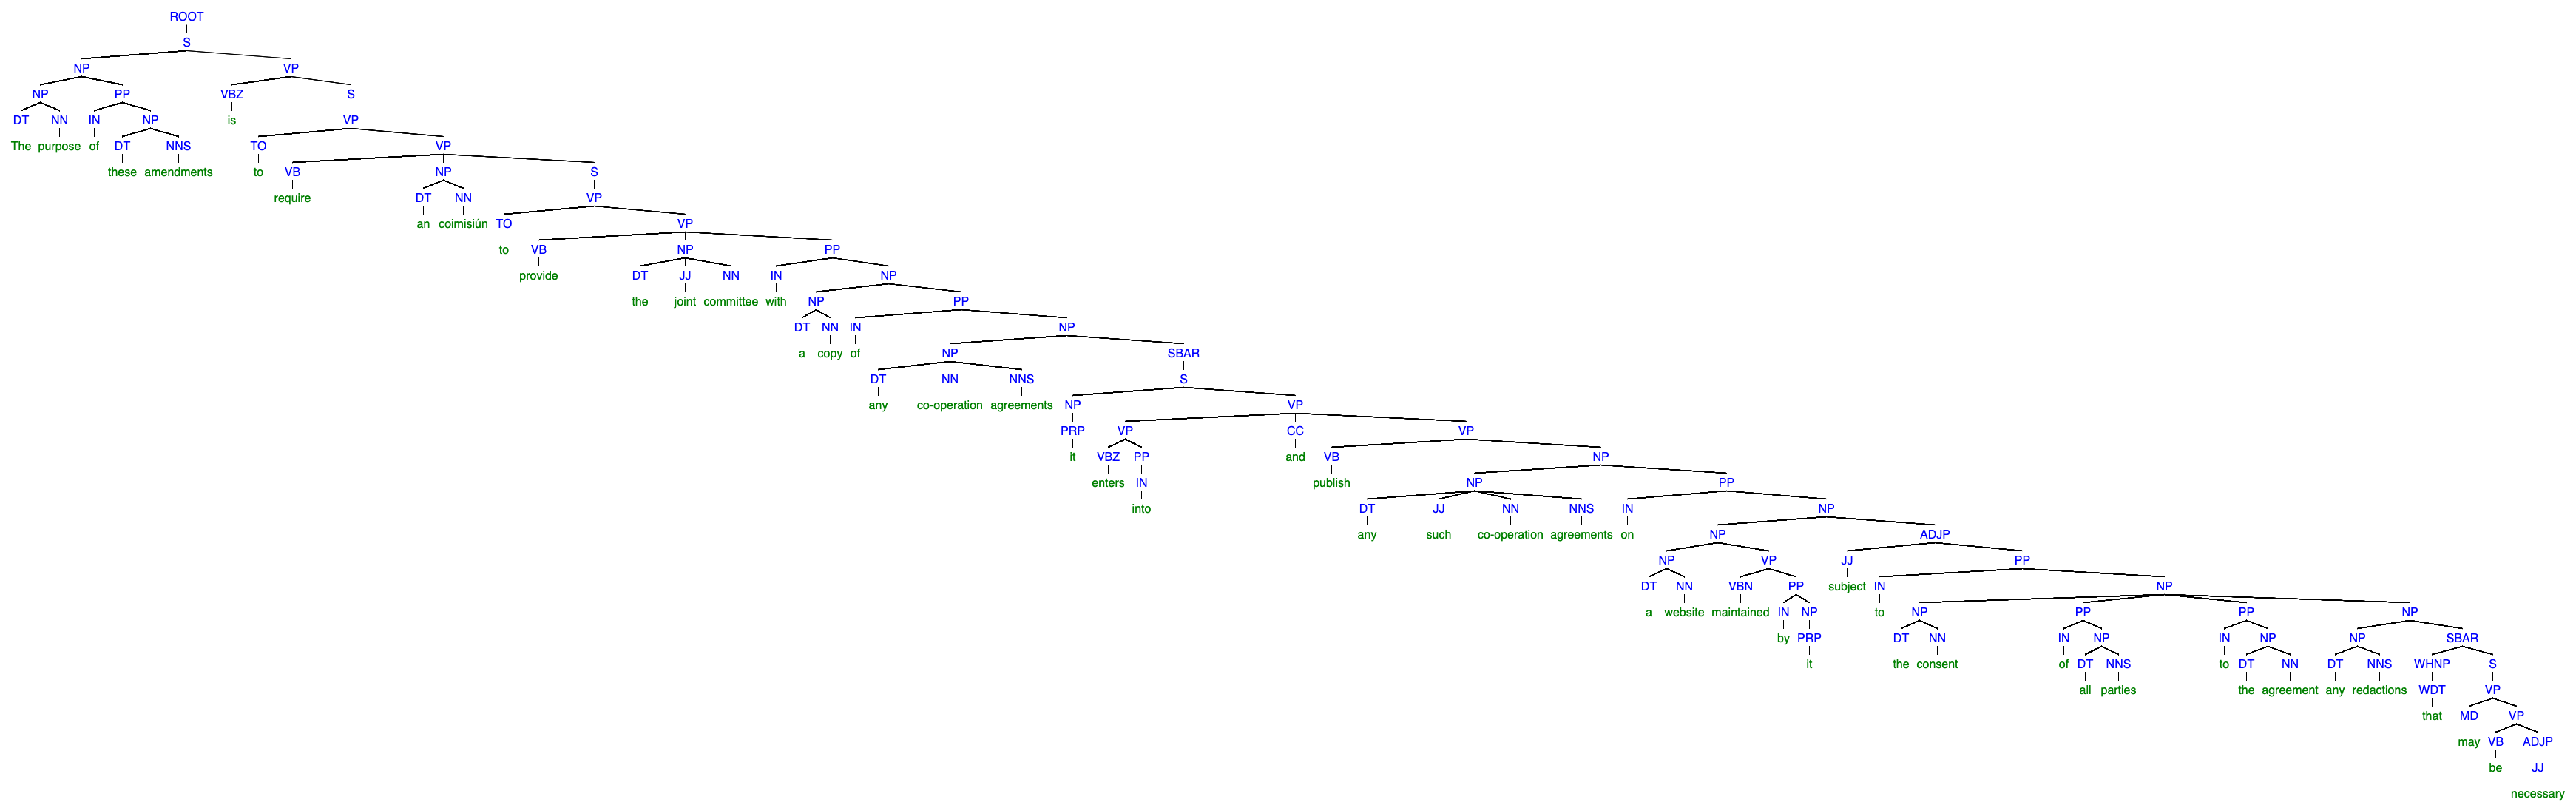
\includegraphics[width=1.0\linewidth]{Dail-Deepest-Tree.png}
\end{figure}
\textbf{Twitter:}
\begin{itemize}
    \item Number of sentences processed = 3525
    \item Mean syntax tree depth = 7.82
    \item Maximum tree depth encountered = 30
    \item Sentence in question: \textit{`People with disabilities and their families deserve to be consulted on decisions that will have such an effect on their ability to access respite and holiday breaks - well done to @savecuisle and @Julie\_ODonoghue for rallying around a service that has done great work for 20 years https://t.co/cOy4REHOWB'}
    \item Tree in question:
    %TC:ignore
    \texttt{(ROOT (S (NP (NP (NNS People)) (PP (IN with) (NP (NP (NNS disabilities)) (CC and) (NP (PRP\$ their) (NNS families))))) (VP (VBP deserve) (S (VP (TO to) (VP (VB be) (VP (VBN consulted) (PP (IN on) (NP (NP (NNS decisions)) (SBAR (WHNP (WDT that)) (S (VP (MD will) (VP (VB have) (NP (NP (PDT such) (DT an) (NN effect)) (PP (IN on) (NP (NP (PRP\$ their) (NN ability) (S (VP (TO to) (VP (VB access) (NP (NN respite)))))) (CC and) (S (NP (NP (NN holiday) (NNS breaks)) (, -) (ADVP (RB well))) (VP (VBN done) (PP (PP (IN to)) (CC and) (PP (IN for) (S (VP (VBG rallying) (PP (IN around) (NP (NP (DT a) (NN service)) (SBAR (WHNP (WDT that)) (S (VP (VBZ has) (VP (VBN done) (NP (JJ great) (NN work)) (PP (IN for) (NP (CD 20) (NNS years)))))))))))))))))))))))))))))))}
    %TC:endignore
    \item As you can see, the generated tree is missing a small number of words from the original sentence due to the removal of @s and links.
\end{itemize}

\begin{figure}[H]
    \centering
    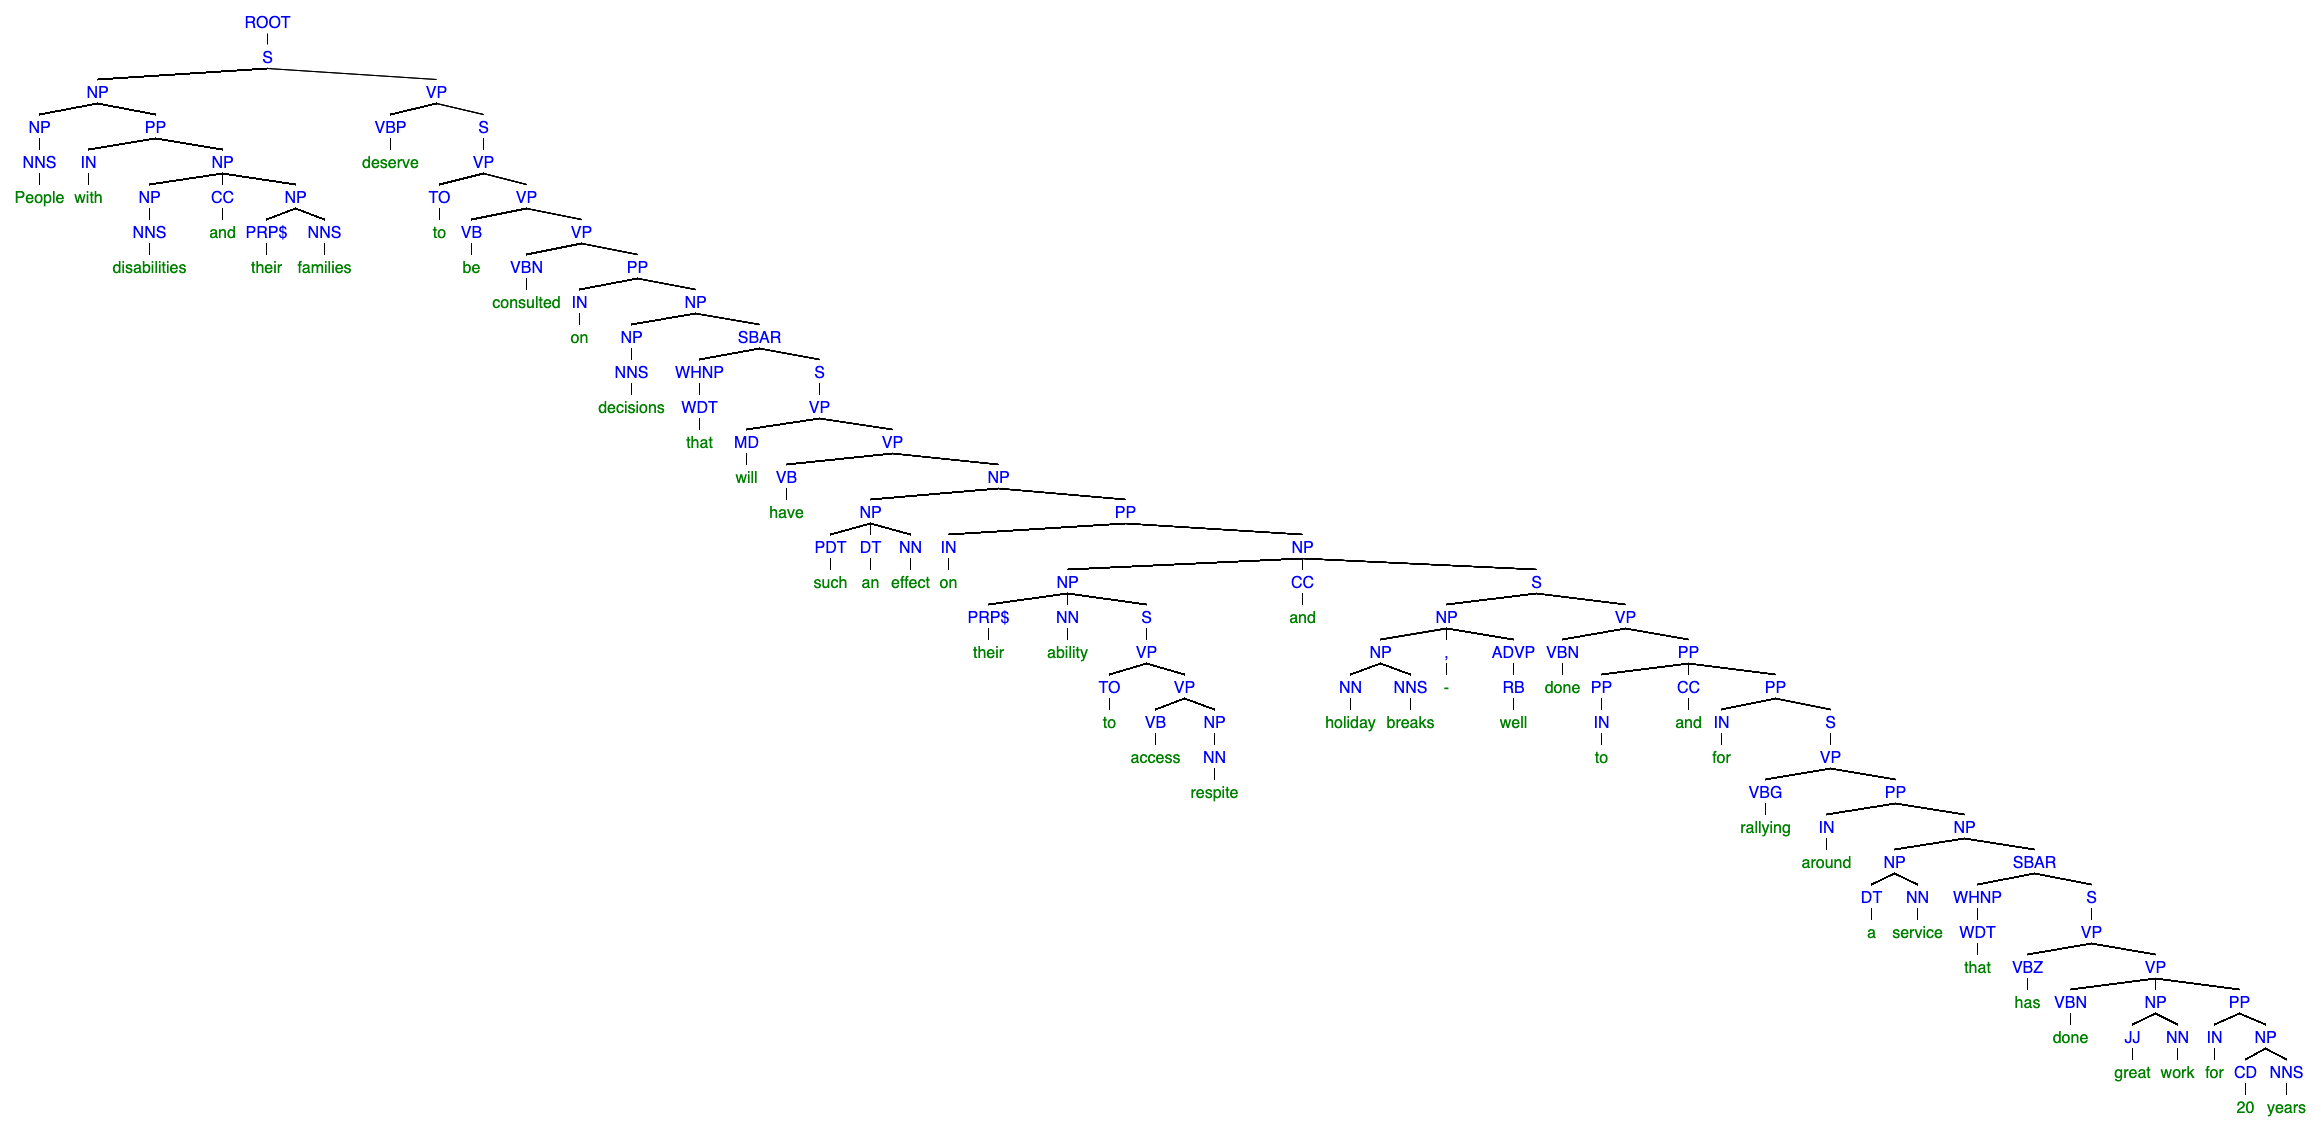
\includegraphics[width=1.0\linewidth]{Deepest-Tree.png}
\end{figure}

\section{Evaluation}
\subsection{Welch Two Sample t-test}
\subsubsection{Word Lengths: Dáil compared to Twitter}
\texttt{t = -0.89405, df = 14038, p-value = 0.3713} \newline
\texttt{alternative hypothesis: true difference in means is not equal to 0} \newline
\texttt{95 percent confidence interval:} \newline
\texttt{-0.15543596  0.05805747} \newline
\texttt{sample estimates:} \newline
\texttt{mean of x mean of y} \newline
\texttt{7.690693  7.739382} \newline
The \textit{p-value} is above 0.05, therefore, there is a significant difference between mean word length depending on the given forum.

 \subsubsection{Tree Depths: Dáil compared to Twitter}
\texttt{t = -3.9486, df = 7101.3, p-value = 7.938e-05} \newline
\texttt{alternative hypothesis: true difference in means is not equal to 0} \newline
\texttt{95 percent confidence interval:} \newline
\texttt{-0.6106279 -0.2054705} \newline
\texttt{sample estimates:} \newline
\texttt{mean of x mean of y} \newline
 \texttt{7.816686  8.224735}
 The \textit{p-value} is not above 0.05, therefore, there is not a significant difference between mean syntax tree depth depending on the given forum.

 \begin{figure}[H]
     \centering
     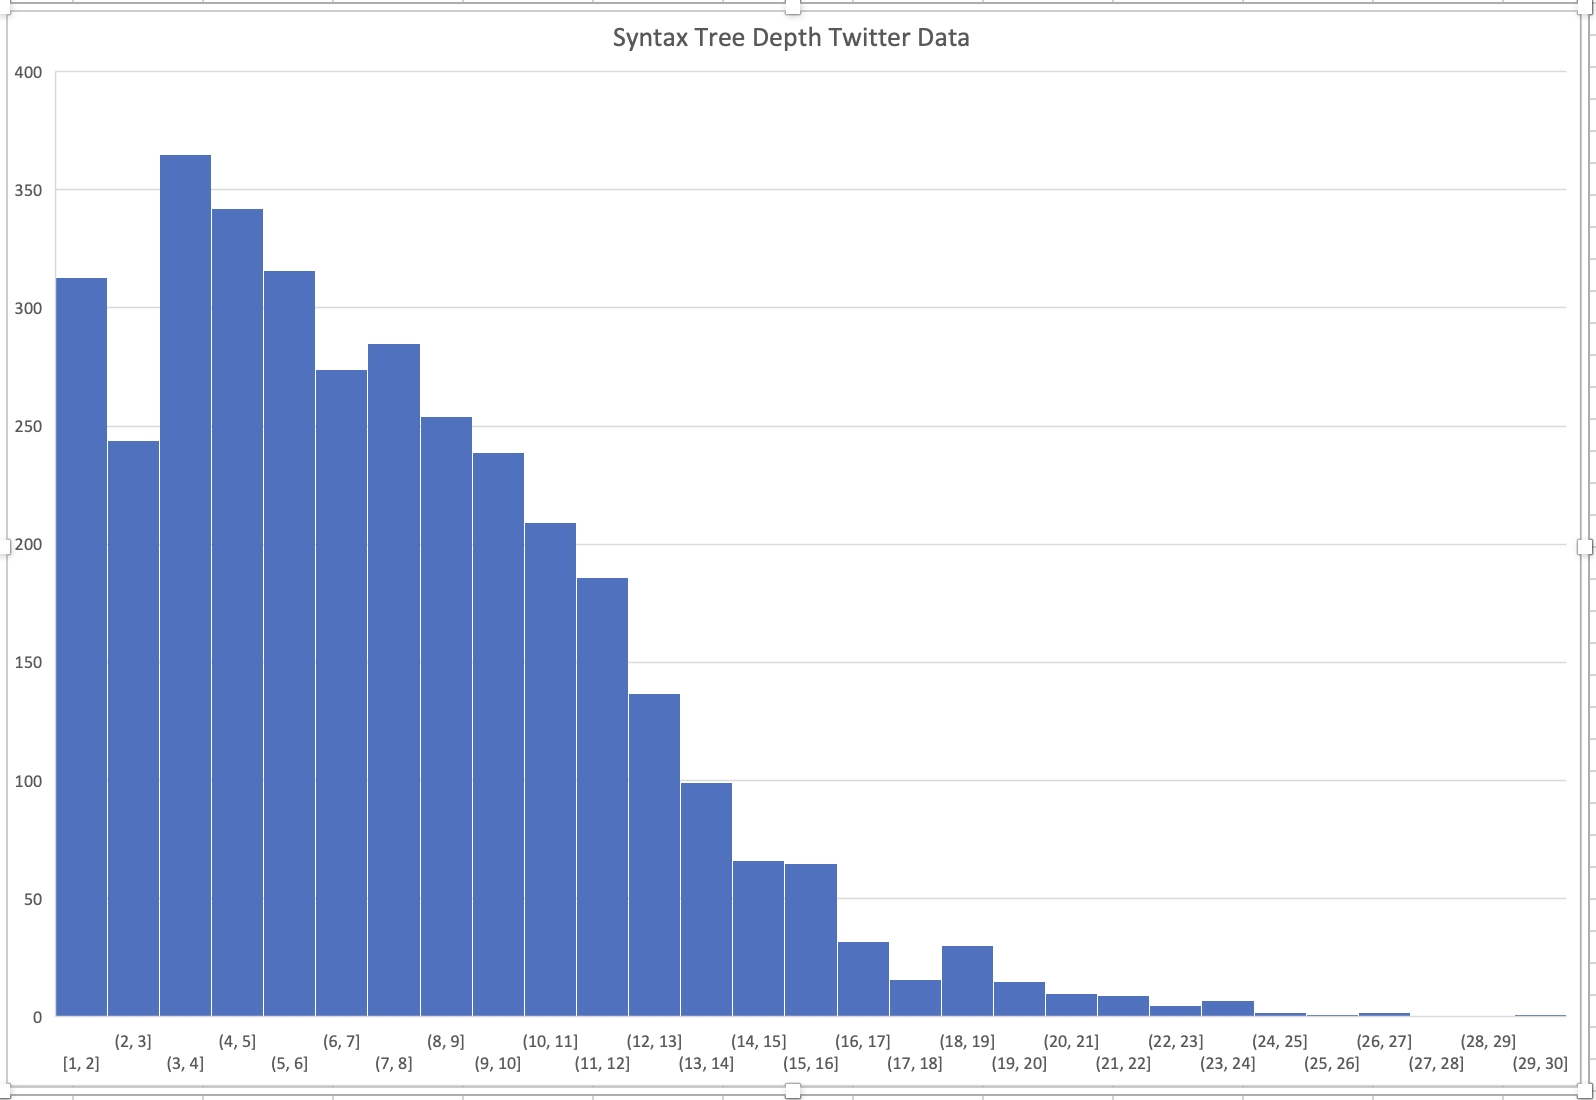
\includegraphics[width=0.5\linewidth]{twitter.png}
     \caption {Distribution of Syntax tree Depths in Twitter}
 \end{figure}

 \begin{figure}[H]
     \centering
     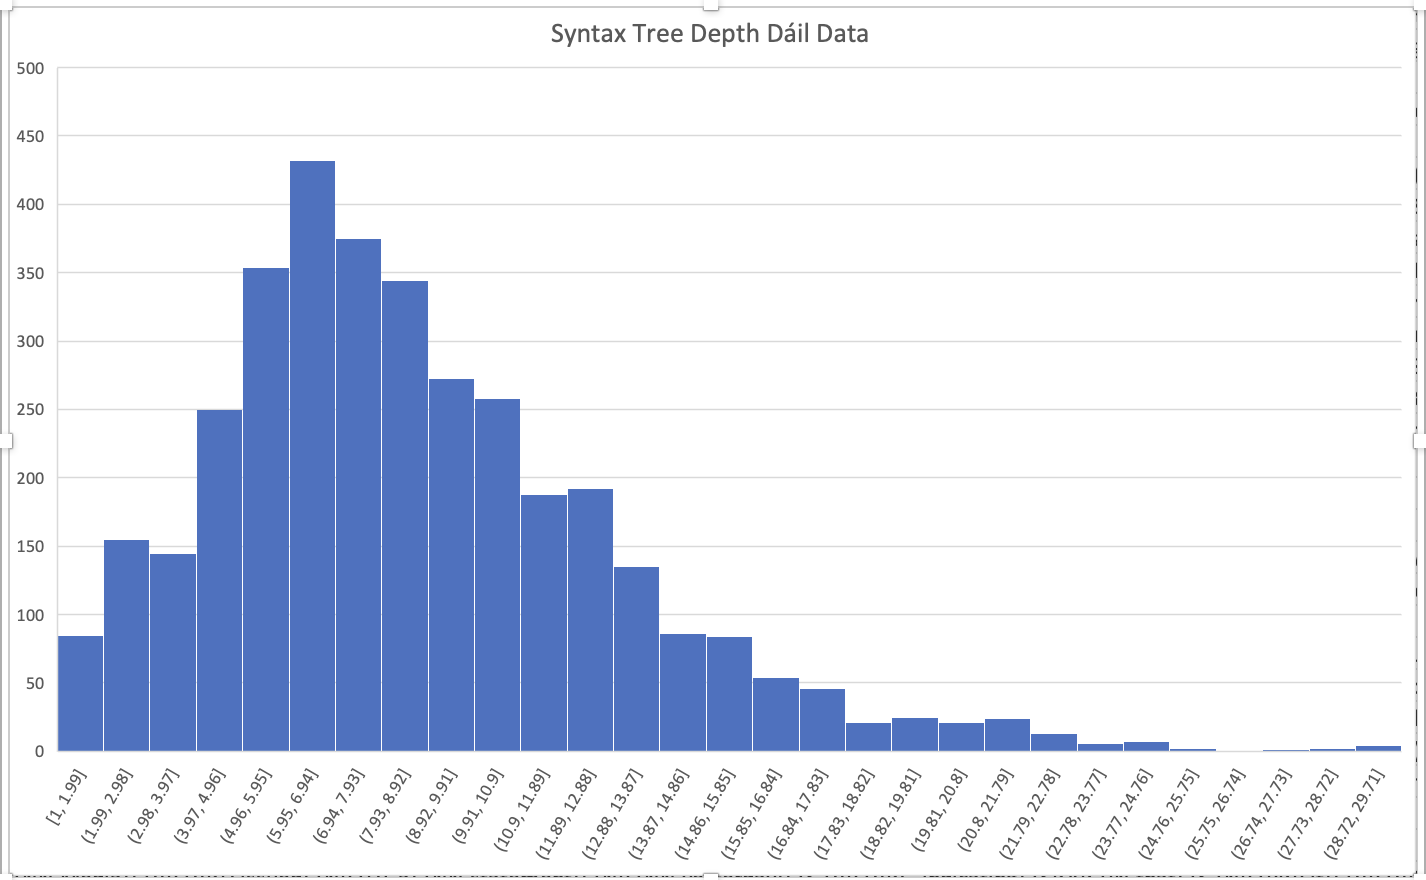
\includegraphics[width=0.5\linewidth]{syntax-tree-dail.png}
     \caption {Distribution of Syntax tree Depths in Dáil}
 \end{figure}


\section{Conclusion}
The \textit{p-value} is above 0.05, therefore, there is a significant difference between mean word length depending on the given forum.
\newline
The \textit{p-value} is not above 0.05, therefore, there is not a significant difference between mean syntax tree depth depending on the given forum.



\bibliographystyle{apalike}
\bibliography{refs}

\begin{appendices}
%TC:ignore
\section{\texttt{C++ code for parsing data into sentences}}
\begin{minted}{c}
#include <iostream>
#include <fstream>
#include <sstream>
#include <string>
#include <vector>
#include <algorithm>

void replace_in_string(std::string &str, std::string &old_str, 
    std::string &new_str); //Not utilised
void remove_emojis(const char** word); //Not utilised
void update_list(std::string &curr_word, int &curr_word_length);

std::vector<std::string> list_words;
std::vector<int> list_lengths;
std::vector<int> list_frequencies;

int main() {
    std::string filename = "TD-Catherine-Martin-Green2.csv";
    std::ifstream file(filename);
    if (!file) {
        std::cerr << "Error opening file " << filename << std::endl;
        return 1;
    }

    std::string line;
    std::vector< std::vector<std::string> > data;

    while (getline(file, line)) {
        std::stringstream ss(line);
        std::vector<std::string> row;
        std::string cell;

        while (getline(ss, cell, ',')) {
            row.push_back(cell);
        }

        data.push_back(row);
    }

    std::vector<std::string> text;
    for (const auto& row : data) {
        text.push_back(row[row.size()-1]);
    }

    int total_word_count = 0;
    int total_word_length = 0;
    int curr_word_length = 0;
    int max_word_length = 0;
    std::string longest_word = "";
    std::vector< std::vector< std::vector<std::string> > > processed_sentenes;

    //For each piece of textual content, remove emojis, #s, @s, etc.
    //Loop through each piece of textual content:
    for (int i = 0; i < text.size(); i++) {
        processed_sentenes.push_back(std::vector< std::vector<std::string> >());
        bool final_sentence = false;
        //Delimit into sentences:
        //Process until ". " or "! " or "? "
        std::string sentences = text[i];
        std::vector<std::string> delims;
        delims.push_back(". ");
        delims.push_back("! ");
        delims.push_back("? ");
        int first_delim = INT_MAX;
        int curr_delim = 0;
        int j = 0;
        while(!final_sentence) {
            processed_sentenes[i].push_back(std::vector<std::string>());
            for (int x = 0; x < delims.size(); x++) {
                curr_delim = sentences.find(delims[x]);
                if (curr_delim != std::string::npos) {
                    first_delim = std::min(first_delim, curr_delim);
                }
            }
            if (first_delim == INT_MAX) {
                final_sentence = true;
                first_delim = text[i].length()-1;
            } else {
            }
            std::string curr_sentence = sentences.substr(0, first_delim);
            char *cstr = new char[curr_sentence.length() + 1];
            strcpy(cstr, curr_sentence.c_str());
            char delim[] = " ";
            const char *token = std::strtok(cstr,delim);
            while(token) {
                //Check for # or @:
                if ((token[0] != '#') && (token[0] != '@')) {
                    //Check for http:
                    std::string curr_word = token;
                    //remove_emojis(&token);
                    if (curr_word.length() >= 4) {
                        std::string first_four = curr_word.substr(0, 4);
                        if (!(first_four == "http")) {
                            curr_word_length = strlen(token);
                            total_word_length += curr_word_length;
                            total_word_count++;
                            max_word_length = std::max(max_word_length, 
                                curr_word_length);
                            if (curr_word_length == max_word_length) {
                                longest_word = token;
                            }
                            update_list(curr_word, curr_word_length);
                            processed_sentenes[i][j].push_back(token);
                        }
                    } else {
                        curr_word_length = strlen(token);
                        total_word_length += curr_word_length;
                        total_word_count++;
                        max_word_length = std::max(max_word_length,
                            curr_word_length);
                        if (curr_word_length == max_word_length) {
                            longest_word = token;
                        }
                        update_list(curr_word, curr_word_length);
                        processed_sentenes[i][j].push_back(token);
                    }
                }
                token = std::strtok(NULL,delim);
            }
            if (!final_sentence) {
                sentences = sentences.substr((first_delim + 1),
                    (sentences.length() - 1));
                first_delim = INT_MAX;
            }
            j++;
        }
    }

    float avg_word_length = (float)total_word_length / (float)total_word_count;
    std::cout << "Total word length = " << total_word_length << std::endl;
    std::cout << "Total word count = " << total_word_count << std::endl;
    std::cout << "Average word length = " << avg_word_length << std::endl;
    std::cout << "Maximum word length = " << max_word_length << std::endl;
    std::cout << "Longest word = \'" << longest_word << "\'" << std::endl;
    std::string all_sentences = "";

    for (int i = 0; i < processed_sentenes.size(); i++) {
        for (int j = 0; j < processed_sentenes[i].size(); j++) {
            std::string sentence = "";
            for (int k = 0; k < processed_sentenes[i][j].size(); k++) {
                std::string word = processed_sentenes[i][j][k];
                if (k != ((processed_sentenes[i][j].size()) - 1)) {
                    sentence += word + " ";
                } else {
                    sentence += word;
                }
            }
            if (i != 0) {
                all_sentences += sentence + "\n";
            }
        }
    }

    std::ofstream MyFile("all_sentences.txt");
    MyFile << all_sentences;
    MyFile.close();
    std::ofstream MyFile2("words_data.csv");
    std::string first_line = "Word,Length,Frequency\n";
    MyFile2 << first_line;
    for (int i = 0; i < list_words.size(); i++) {
        std::stringstream ss;
        ss << list_lengths[i];
        std::string length;
        ss >> length;
        std::stringstream ss2;
        ss2 << list_frequencies[i];
        std::string frequency;
        ss2 >> frequency;
        std::string next_line = list_words[i] + "," + length +
            "," + frequency + "\n";
        MyFile2 << next_line;
    }
    MyFile2.close();
    return 0;
}

void replace_in_string(std::string &str, std::string &old_str, 
    std::string &new_str) { //Not utilised
    for(std::size_t pos = str.find(old_str); pos != std::string::npos;
        pos = str.find(old_str, pos))
        {
            str.replace(pos, old_str.size(), new_str);
            pos += new_str.size();
        }
}

void remove_emojis(const char** word) { //Not utilised
    std::string new_word; //Word with emojis removed
    *word = new_word;
}

void update_list(std::string &curr_word, int &curr_word_length) {
    bool already_exists = false;
    for (int i = 0; i < list_words.size(); i++) {
        //If curr_word in list
        if (list_words[i] == curr_word) {
            already_exists = true;
            list_frequencies[i]++;
        }
    }
    //If curr_word not in list
    if (!already_exists) {
        list_words.push_back(curr_word);
        list_lengths.push_back(curr_word_length);
        list_frequencies.push_back(1);
    }
}
\end{minted}
\section{\texttt{Python code for generating trees}}
\begin{minted}{python}
import stanza
stanza.download('en') # download English model
nlp = stanza.Pipeline('en') # initialize English neural pipeline
#Pre-processed input data:
#Twitter: "Twitter_processed_sentences.txt"
#Dáil: "Dail_processed_sentences.txt"
f = open("Twitter_processed_sentences.txt", "r")
overall_depth = 0
num_sentences = 0
overall_max_depth = 0
line_index = 1
#Total lines of input data:
#Twitter: 3211
#Dáil: 3548
total_lines = 3211
overall_max_depth_sentence = ""
#Output file name:
#Dáil: "./Output/Dail-Trees-Depth.csv"
#Twitter: "./Output/Twitter-Trees-Depth.csv"
file_name = "./Output/Twitter-Trees-Depth.csv"
newfile = open(file_name, "x")
newfile.write("Tree,Max-Depth\n")
for sentence in f:
    percent_complete = 100*(line_index / total_lines)
    print("Processing line", line_index, "of", total_lines, "| Percentage
        complete:", percent_complete, "%")
    doc = nlp(sentence) # run annotation over a sentence
    max_depth = 0
    curr_depth = 0
    for sentence in doc.sentences:
        tree = sentence.constituency
        newfile.write(str(tree) + ",")
        for child in tree.children:
            curr_depth = child.depth()
            max_depth = max(max_depth, curr_depth)
            overall_max_depth = max(overall_max_depth, max_depth)
            if curr_depth == overall_max_depth:
                overall_max_depth_sentence = sentence
        newfile.write(str(max_depth) + "\n")
        overall_depth += max_depth
        num_sentences += 1
    line_index += 1
overall_depth_avg = overall_depth / num_sentences
print("Number of sentences processed = ", num_sentences)
print("Average syntax tree depth = ", overall_depth_avg)
print("Maximum tree depth encountered = ", overall_max_depth)
print("Sentence in question = ", overall_max_depth_sentence)
print("Tree of sentence in question = ", overall_max_depth_sentence.constituency)
newfile.close()
\end{minted}
%TC:endignore
\end{appendices}
%\nocite{*} %includes all references in bibliography, even if not explicitly cited in the text
\end{document}
